\documentclass[11pt]{article}
\usepackage[top=1in, bottom=1in, left=1in, right=1in]{geometry}
\parindent 22pt

\usepackage{amsmath}
\usepackage{amsfonts}
\usepackage{amssymb}
\usepackage{bm}
\usepackage{etoolbox}
\usepackage{graphicx}
\usepackage{tabularx,ragged2e,booktabs,caption}
\usepackage{caption}
\usepackage[none]{hyphenat}
\usepackage{booktabs,caption,fixltx2e}
\usepackage[para]{threeparttable}
\usepackage[capposition=top]{floatrow}
\usepackage{caption}
\usepackage{subcaption}
\usepackage{pdfpages}


\begin{document}


\includepdf[pages={1}]{ConsumptionEarnings1.pdf}

\includepdf[pages={1}]{ConsumptionEarnings3.pdf}
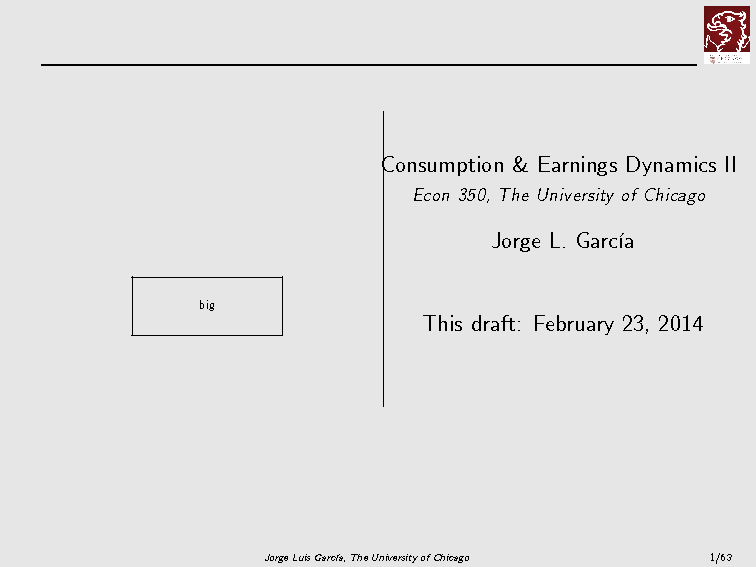
\includepdf[pages={1}]{ConsumptionEarnings2.pdf}

\end{document}




